\section{attic}

\textbf{stuff we don't want to get rid of but don't know what to do with}

\subsection{Kinds of Relations}
    
%%\jmh{Ack ... deductive rules are unsafe, and technically Datalog-neg forbids them due to the free variable in the head.  So you will need to expand your language to include an acceptable notion of per-timestep safety (as Maier suggested), at which point it's not a subset of Datalog-neg.  Would be nice to be able to say ``\lang is a subset of (Datalog + \{set of addons\})'' but that would require defining the acceptable saftey before defining timestamps (which are a restriction).}
%\nrc{Title is too long: EDB, IDB, and NDB instead?}
In a \lang program, there are three kinds of relations:
extensional, {\em intensional} or {\em nondeterministic}.

%\nrc{We define the term ``extensional predicate'' before, but not
%  ``extensional relation''.}
\begin{definition}
%
An \emph{intensional} relation is a relation that appears
in the head of one or more atemporal or inductive rules in the program, but
never in the head of an asynchronous rule.~\nrc{``atemporal'' rules
  have not been defined.}
%
\end{definition}
\begin{definition}
%
A \emph{nondeterministic} relation is a relation that
appears in the head of one or more asynchronous rules in the program.
%
\end{definition}
We refer to the sets of ground atoms in intensional and nondeterministic
predicates respectively as the IDB, and NDB.

%\jmh{introduction of the MDB doesn't seem useful, actually.  I'd drop this,
%and if you need to define a ``mutable'' relation as one that participates in
%the head of a temporal rule, you can do so as needed.}
The EDB, IDB, and NDB are all pairwise disjoint.  Intuitively, the distinction
between the NDB and IDB is that the NDB is determined nondeterministically~\nrc{clumsy} from
the EDB, IDB and NDB, while the IDB is determined deterministically from the
EDB, IDB and NDB.  Thus, given a \lang instance, all IDB predicates that do
not transitively depend on NDB predicates can be evaluated deterministically.
We will refer to facts, ground atoms in the EDB, and \emph{events}
interchangeably, for reasons which will soon become clear.
%%\jmh{The only reason to worry about the MDB being non-deterministic is @sync, which you didn't in fact need to introduce yet.  Again, I don't see this discussion being useful.}

\subsection{Traces}


\begin{figure}[t]
  \centering
  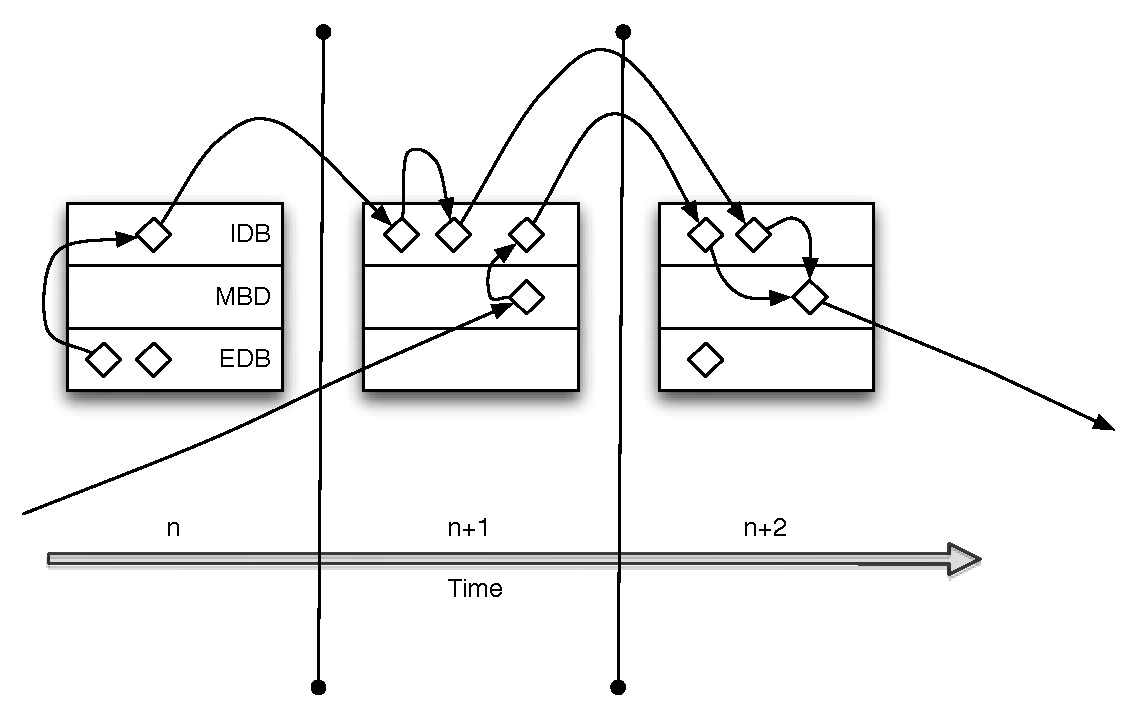
\includegraphics[width=1\linewidth]{figures/edbidbmdb.pdf}
  \label{fig:edbidbmdb}
  \caption{Derivations across time in IDB and MDB relations.}
\vspace{-8pt}
\end{figure}

\paa{this section (its placement \emph{and} content) is somewhat problematic given the current structure
of the draft.  We've established the notion of finite preambles of a (possibly infinite) EDB.  A trace is basically just
an interpretation (a set of ground atoms) -- by calling it a ``trace" we're connoting a post-hoc \wrm{warning: post hoc is undefined} interpretation.
A trace that is just EDB is sufficient, given a program, to augment the trace with IDB and MDB atoms such that
the resulting trace is a model (by simply running a fixpoint computation).  For a program with no async rules, the EDB of input is sufficient to recreate the
program execution exactly -- that is to say, to reproduce the single minimal model of the program given the EDB.
It is \emph{not} sufficient to recreate the execution of a program with async rules: intuitively, we'd need to include in 
the trace the complete MDB, for every entry in it potentially corresponds to one of many possible minimal models.
perhaps we just want to show that there is a method (drop the async rules and run a fixpoint computation to generate
the IDB from MDB and EDB) to regenerate a "complete trace" (ie minimal model) from EDB $\cup$ MDB}

%Consider a non-empty EDB $E$, an empty MBD $M$ and IDB $I$ and a program $P$.  Evaluating $P$ against $E$ may derive facts in $M$ and $I$.

\begin{definition}
A \emph{trace} is any set of facts from the EDB, NDB or IDB of a \lang program evaluation.
\end{definition}

Any trace for a \lang instance $(P,E)$ is an interpretation of $(P,E)$.
%\wrm{lol, why do we need the notion of an incomplete trace?}

\begin{definition}
%
A \emph{complete trace} of an evaluation of a \lang instance is the union of
the given EDB with the derived IDB and MDB.
%
\end{definition}

\begin{lemma}
%
A complete trace of a \lang instance $(P,E)$ is its unique minimal model.
%
\end{lemma}

%\begin{lemma}
%%
%For any bound on $successor$, a complete trace of a \lang  instance $(P,E)$ has a unique minimal model.
%%
%\end{lemma}

If we evaluate E given P, and P is stratifiable, the resulting set of ground atoms is a minimal model.
In our case, however, successor causes our EDB to be infinite, so the minimal model of any \lang program 
with temporal rules is potentially infinite.  \paa{but we'd like to show that a weaker property holds: that for any value $N$
in the \emph{successor} relation, the resulting program has a minimal model.}
\wrm{we either already showed this, or our theorems above are wrong.}


\begin{definition}
A \emph{minimal trace} is a subset of a complete trace that excludes any IDB ground atoms derived through an inductive
rule.
\end{definition}

A minimal trace of a \lang program $P$ is equivalent to the complete trace of which is is a subset -- the latter may be derived from the former by repeated
applications of inductive rules.  However, a given a \lang instance $(P, E)$ and a minimal trace T (where $E \subset T$), a fixpoint
computation will most likely \emph{not} yield a minimal model, because new tuples may be added to the MDB that represent a component 
of a different minimal model, and because these may affect the IDB.  The set of ground atoms $EDB \cup MDB_{old} \cup IDB_{new}$
\emph{may} may be a minimal model, iff $IDB_{new} = IDB_{old}$.  \paa{actually I am not sure if that is true}.  
$(EDB \cup MDB_{old} \cup IDB_{new} \cup IDB_{old})$ is certain to be a model, but is only minimal if $IDB_{new} \subset IDB_{old}$.

A minimal trace records the nondeterminism caused by the delay or reordering of async rules, and
is equivalent to the original program execution.  

\begin{definition}
A \emph{reduced trace} is a minimal trace with normalized time suffixes starting with 0 and increasing by 1 at each step.
\end{definition}

show a (trivial) procedure for reduction and make some claims about equivalences without entanglement.

\begin{definition}
A \emph{event trace} is a \lang EDB.
\end{definition}

An event trace and program P may be used to generate a new IDB and MDB.  The MDB is virtually certain to differ from that of another
execution, while the IDB may differ, depending on its dependency on the MDB.  The union of these three databases is of course a
minimal model, but probably not the same minimal model from another execution.  \paa{but can we say that it will often be true that if we project 
out the time attribute from every predicate, the minimal models will be the same? it won't always be true...}



\subsection{EDB Preambles}

\rcs{I've never seen someone use ``preamble'' to refer to this concept.  Why not call it a prefix?}

A \slang instance's EDB may be arbitrarily large.  In this section we introduce
the notion of a {\em preamble} -- a truncation of the EDB, and prove an
equivalence between full evaluation of a preamble and incremental evaluation
based on evaluation of an earlier preamble.
%A \slang instance may receive arbitrarily many external input tuples over the
%course of its execution, but should not wait arbitrarily long before
%performing deductions.  In this section we introduce the notion of EDB
%preambles, and prove an equivalence between two types of evaluation.

%In general, the EDB of a \slang instance may be infinite, and may lead to unsafe evaluations even when \emph{successor} is derived from it
%as in a post-hoc evaluation.

\begin{definition}
A \emph{preamble} $\alpha_{n}$ of an EDB $\Gamma$ is the set of facts in $\Gamma$ whose timestamp is less than or equal to $n$.
\end{definition}

If the EDB is finite, then it has a maximum timestamp $\top$, \rcs{is successor now part of the EDB? Otherwise, there is no max timestamp} and
$\alpha_{\top}$ = $\Gamma$.  \wrm{I don't think we use $\top$ anywhere else}
Because each preamble is a superset of all preambles with lower indices, we
have the monotonicity property:

$\forall \alpha_{i}, \alpha_{j} \in \Gamma : (i < j) \to (\alpha_{i} \subseteq \alpha_{j})$

%\paa{to your point, bill, I switched the lemma and proof below to one of IDB equivalence in the posthoc vs. continual interpretation
%rather than an inductive proof that every model in the series is minimal.  there is probably a very similar proof of the latter
%that we could include in the next section after introducing minimal models, stratification etc}

\wrm{todo: disuss replacing FP with some derivation tree thing}
\begin{definition}
%
Let $F$ be the set of all finite subsets of possible atoms.  Let $P$ be the set
of all finite subsets of possible rules.  Let $FP : P \times F \mapsto F$ be
the function representing the \emph{fixpoint} computation carried out by a
datalog interpreter.  That is, $FP_p$ takes an EDB to its corresponding IDB.
%
\end{definition}


\begin{lemma}
\label{lem:costmodel}
%
Let $i \in \mathbb{Z}$.  Then, $FP_p(\alpha_{i+1} \cup FP_p(\alpha_i)) =
FP_p(\alpha_{i+1})$.
%
\end{lemma}

%%this could (with some work) lead to an inductive proof
%%that an infinite model is minimal.  we could prove the (weaker?) property that
%%the infinite series of models of increasing finite preambles of an EDB are all 
%%minimal if one of them is.

\begin{proof}

%%Inductive step:

%%if we assume that some program P and finite preamble $\alpha_n$ of a trace $\Gamma$ produce a minimal model, 
%%then it follows that a preamble $\alpha_{n+1}$ and the IDB produced by the previous model produce a minimal model.

by contradiction. Assume $\exists i \in \mathbb{Z}$ such that:
$FP_p(\alpha_{i+1} \cup FP_p(\alpha_i)) \neq FP_p(\alpha_{i+1})$

{\bf Case 1:} $\exists A \in FP_p(\alpha_{i+1} \cup FP_p(\alpha_i)) : A \not\in FP_p(\alpha_{i+1}).$

This implies that $A$ is transitively dependent on atoms in $\alpha_{i+1} \cup
FP_p(\alpha_i)$.  However, if $A$ is transitively dependent only on atoms in
$\alpha_{i+1}$, then $A$ would be in $FP_p(\alpha_{i+1})$.  Thus, $A$ must be
transitively dependent on some atoms in $FP_p(\alpha_{i})$.  But $\alpha_{i}
\subset \alpha_{i+1}$, so this implies that $A$ is transitively dependent on
some atom in $\alpha_{i+1}$, which means $A \in FP_p(\alpha_{i+1})$.  This
contradicts our assumption, thus no such $A$ may exist.

{\bf Case 2:} $\exists A \in FP_p(\alpha_{i+1}) : A \not\in FP_p(\alpha_{i+1} \cup FP_p(\alpha_i)).$

This implies that $A$ is transitively dependent on $\alpha_{i+1}$.  In order
for $A \not\in FP_p(\alpha_{i+1} \cup FP_p(\alpha_i))$, we need $A$ to depend
negatively on an atom $B \in FP_p(\alpha_i)$.  But $B$ transitively depends on
an atom $C \in \alpha_i$.  $C \in \alpha_{i+1}$ by definition (if $B$ is
extensional, then $C=B$), so $B \in FP_p(\alpha_{i+1})$, so $a \not\in
FP_p(\alpha_{i+1})$.  This contradicts our assumption, thus no such $A$ may
exist.
%If $I_2 \neq I_3$, it must be the case that either there exists a ground atom in $I_2$ that is not in $I_3$, or that is in
%$I_3$ and not in $I_2$.  
%Take the former case first.  This means there is an atom $A$ that is entailed by P given $FP(\alpha_{j} \cup FP(\alpha_{i}))$
%but not entailed by P given $\alpha_{j}$, so it must be in $I_1$.   The only circumstances under which an atom in
%$I_1$ would not occur in the IDB $FP(\alpha_{j})$ is if there is a fact $B$ in $\alpha_{j}$ 
%corresponding to a negated subgoal in a rule $r$ in P upon which $A$ depends.  However, for this to occur, because a ground atom 
%in $I_1$ cannot depend upon a ground atom from the ``future", that fact $B$ would need to have occurred at some time less than 
%or equal to the to timestamp of atom $A$.  But this is not possible, because all timestamps in $\alpha_{j}$ that are not in any $\alpha_{k} | k<j$
%are strictly higher than any timestamps in $\alpha_{k}$.  Hence the first case leads to contradiction.
%As for the second case...
\end{proof}

\subsection{Cost Model}
%%\newdef{definition}{Definition}
Lemma~\ref{lem:costmodel} implies that we can trade computation cost for
storage cost in evaluation of a \slang program. 

%In the continuous interpretation of a \slang program, it is in general only
%useful to remember facts at a single timestamp in a predicate.  Two ways to
%approach this issue are to either always persist the ``latest'' version, or
%continuously re-derive the latest version.  These are represented in the naive
%deductive and overwriteable storage implementations below.

%\begin{figure}[t]
%\begin{tabular}{ll} \hline
%%Rule Pattern & Idiom & Prepare & Propose & Election \\ \hline \hline
%$d$ & Cost of a deductive step \\
%$s$ & Cost of storing a tuple \\
%$r$ & Cost of reading a tuple \\ 
%$t$ & Number of tuple derivations from deductive rules \\ 
%\hline
%$S$ & Set of tuples inserted \\
%$U$ & Set of tuples updated \\
%$P$ & Set of stored tuples, with time projected out \\ 
%$T$ & Set of stored tuple timestamps \\ 
%$Q$ & Set of query timestamps \\ \hline 
%\end{tabular}
%\caption{Cost model.}
%\label{fig:breakdown}
%\end{figure}


%\subsubsection{Naive Deductive Implementation}

%To evaluate a trace consisting of $S$ inserts and $U$ updates, a naive
%deductive implementation would:

%\begin{enumerate}
%
%\item
%
%\item
{\bf Naive Deductive Implementation: } We must evaluate every rule at time $1$
through $M$.  This implies persistent storage cost of $|\alpha_M|$, e.g. the
entire preamble up through $M$.
%A bottom-up evaluation of a predicate $P$ consists of evaluating all rules
%that reference $P$ in the head, and may involve polynomially many derivations
%in the size of the EDB up to time $M$.
A naive query plan for execution of a rule $R$ would take the cross product of
all body relations, $CP_R$, select the subset that matches the body conditions,
and project this subset onto the head predicate.  Assume each rule $R$ has an
associated selectivity from the cross product $s_R$, cost per each tuple in the
cross product $d_R$, and cost per each tuple in the subset selected from the
cross product $p_R$.  Each recursion is executed for a certain number of steps
steps.  This step has temporary storage and execution cost of:
%
\[ \sum_{t=0}^M \sum_{R} |CP_{(R,t)}|(p_{(R,t)} \cdot s_{(R,t)} + \cdot
d_{(R,t)}) \]
%
%\end{enumerate}

%In summary, the total execution cost is:

%\[ (S+2U)w + M \cdot \sum_{r : P \in r.head} n_r \cdot s_r \cdot d_r  \]

%Since we only need persist the EDB, the total storage cost is equal to the size
%of the EDB.

%$(|S|+2|U|)s + (|S|+2|U|)r + t + (\displaystyle\sum_{i=0}^{|Q|-1} \displaystyle\sum_{j=0}^{|T|-1} Q_{i} - T_{j})d$

%\subsubsection{Naive Overwriteable Storage Implementation}

%To evaluate a trace consisting of $S$ inserts and $U$ updates, a naive
%deductive implementation would:

%\begin{enumerate}
%
%\item
%Add all $I$ inserts, $D$ deletions, and $U$ updates to a log.  Note that
%an update consists of both an insertion and a deletion.  Assuming that
%inserting a fact into the EDB has some cost $w$ independent of the
%characteristics of the predicate (e.g. all predicates store their facts in hash
%tables), then this step has temporary storage and computation cost $(I+D+2U)w$.

{\bf Naive Overwriteable Storage Implementation: }An overwritable storage
implementation may trade some storage for better execution latency by storing
the most recent version of all predicates.  This implies persistent storage
cost of:
%
\[ |FP(\alpha_{M-1})| + |\alpha_M \cap \alpha_{M-1}| \]

We would need to evaluate every rule $R$ at timestamp $M$.  This entails
temporary storage and execution cost of:
%
\[ \sum_{R} |CP_{(R,M)}|(p_{(R,M)} \cdot s_{(R,M)} + d_{(R,M)}) \]
%This is in contrast to the
%naive deductive model, which would require computation from timestamp 1, but
%would not require persisting the IDB of the most recently computed stratum for
%each predicate.

%In summary, the total execution cost is:

%\[ (S+2U)w + \sum_{r} (M - Q_{r.head}) n_r \cdot s_r \cdot d_r  \]

%The total storage cost is the IDB of each predicate at its most recent
%timestamp.

%%\subsubsection{perhaps we can admit queries over the past that are bounded and pre-stated, and do GC}


